\documentclass[aspectratio=169, 11pt]{beamer}

\usepackage[utf8]{inputenc}
\usepackage{graphicx}
\usepackage{tikz}
\usetikzlibrary{positioning}
\usepackage{xcolor}
\usepackage{amsmath}
\usepackage{amssymb}
\usepackage{listings}
\usepackage{array}
\usepackage{booktabs}
\usepackage{colortbl}
\usepackage{pifont}

% ---- Modern color scheme ----
\definecolor{primary}{RGB}{15, 40, 70}       % deep navy
\definecolor{secondary}{RGB}{25, 92, 124}    % industrial blue
\definecolor{accent}{RGB}{41, 197, 180}      % teal accent
\definecolor{highlight}{RGB}{255, 172, 58}   % warm amber
\definecolor{light}{RGB}{239, 245, 249}       % soft background
\definecolor{mid}{RGB}{220, 228, 235}        % mid gray
\definecolor{dark}{RGB}{31, 35, 40}           % near black
\definecolor{panel}{RGB}{247, 250, 252}       % panel color

% ---- Beamer theme setup ----
\usetheme{default}
\usecolortheme{default}
\setbeamercolor{normal text}{fg=dark,bg=white}
\setbeamercolor{structure}{fg=secondary}
\setbeamercolor{title}{fg=primary}
\setbeamercolor{subtitle}{fg=secondary}
\setbeamercolor{frametitle}{fg=white,bg=primary}
\setbeamercolor{block title}{bg=primary,fg=white}
\setbeamercolor{block body}{bg=panel,fg=dark}
\setbeamercolor{item projected}{bg=accent,fg=white}
\setbeamercolor{alerted text}{fg=highlight}
\setbeamercolor{example text}{fg=secondary}
\setbeamerfont{frametitle}{size=\Large,series=\bfseries}
\setbeamerfont{title}{size=\fontsize{30}{34}\selectfont,series=\bfseries}
\setbeamerfont{subtitle}{size=\large,series=\bfseries}
\setbeamertemplate{navigation symbols}{}
\setbeamertemplate{itemize item}{\textcolor{accent}{\ding{108}}}
\setbeamertemplate{itemize subitem}{\textcolor{secondary}{\ding{117}}}
\setbeamertemplate{frametitle}{%
  \nointerlineskip
  \begin{beamercolorbox}[wd=\paperwidth,ht=2.7em,dp=0.6em,leftskip=0.8em,sep=0.25em]{frametitle}
    \usebeamerfont{frametitle}\insertframetitle
  \end{beamercolorbox}
}
\setbeamertemplate{footline}{%
  \leavevmode%
  \hbox{%
    \begin{beamercolorbox}[wd=.34\paperwidth,ht=2.5ex,dp=1ex,leftskip=1em]{author in head/foot}
      \insertshortauthor
    \end{beamercolorbox}%
    \begin{beamercolorbox}[wd=.32\paperwidth,ht=2.5ex,dp=1ex,center]{title in head/foot}
      \insertshorttitle
    \end{beamercolorbox}%
    \begin{beamercolorbox}[wd=.34\paperwidth,ht=2.5ex,dp=1ex,rightskip=1em,sep=0pt]{date in head/foot}
      \insertframenumber{}/\inserttotalframenumber
    \end{beamercolorbox}%
  }%
  \vskip0pt%
}
\setbeamercolor{author in head/foot}{bg=secondary,fg=white}
\setbeamercolor{title in head/foot}{bg=primary,fg=white}
\setbeamercolor{date in head/foot}{bg=secondary,fg=white}
\setbeamertemplate{background}{
  \begin{tikzpicture}[remember picture,overlay]
    \fill[light] (current page.south west) rectangle (current page.north east);
    \fill[secondary!10] (current page.north west) rectangle ([xshift=0.55\paperwidth,yshift=-0.18\paperheight]current page.north east);
    \fill[accent!18] ([xshift=0.73\paperwidth,yshift=-0.02\paperheight]current page.north west) rectangle ([xshift=\paperwidth,yshift=-0.22\paperheight]current page.north east);
    \draw[secondary!25, line width=0.4pt] ([xshift=0.05\paperwidth,yshift=0.06\paperheight]current page.south west) grid[step=0.7cm] ([xshift=-0.05\paperwidth,yshift=-0.06\paperheight]current page.north east);
  \end{tikzpicture}
}

\newcommand{\emphred}[1]{\textcolor{secondary}{#1}}
\newcommand{\emphhighlight}[1]{\textcolor{primary}{\textbf{#1}}}

\title{SolSight}
\subtitle{\emphred{Solder Defect Detection System} --- Automatic Optical Inspection with AI}
\author{AI-Powered Defect Detection}
\date{\today}

\begin{document}

%==================== SLIDE 1: TITLE SLIDE ====================
\begin{frame}[plain]
    \begin{tikzpicture}[remember picture,overlay]
        \fill[primary] (current page.north west) rectangle ([yshift=-2.9cm]current page.north east);
        \fill[accent] ([xshift=0.52\paperwidth,yshift=-0.8cm]current page.north west) rectangle ([xshift=0.84\paperwidth,yshift=-2.9cm]current page.north east);
        \fill[highlight!75] ([xshift=0.1\paperwidth,yshift=-1.6cm]current page.north west) rectangle ([xshift=0.35\paperwidth,yshift=-2.6cm]current page.north east);
    \end{tikzpicture}

    \vspace*{1.5cm}
    \begin{center}
        {\fontsize{30}{34}\selectfont\bfseries\color{white} SolSight}

        \vspace{0.45cm}

        {\large\color{accent}\textbf{Solder Defect Detection System}}

        \vspace{0.7cm}

        {\large\color{white} Unsupervised Anomaly Detection for PCB Assembly}

        \vspace{0.8cm}

        \begin{beamercolorbox}[wd=0.82\paperwidth,rounded=true,shadow=true,leftskip=1em,sep=0.7em]{block body}
            \begin{itemize}
                \item \emphhighlight{Fully Convolutional Autoencoder} for real-time inspection
                \item \emphred{Resolution-Agnostic} architecture (16px to 160px)
                \item \emphred{Zero-Supervised} learning on defect-free joints
            \end{itemize}
        \end{beamercolorbox}
    \end{center}
\end{frame}

%==================== SLIDE 2: THE PROBLEM ====================
\begin{frame}{\emphred{The Problem}}
    \vspace{0.5cm}
    \begin{itemize}
        \item Manual solder joint inspection is \emphred{time-consuming \& error-prone}
        \item Defects \& degradation in PCB assemblies directly impact reliability
        \item Traditional AOI systems require \emphred{extensive labeled datasets}
        \item Defect variations across hardware make generalization \emphred{difficult}
    \end{itemize}

    \vspace{1cm}
    \begin{center}
        \textbf{\large What if we could detect anomalies without labeling defects?}
    \end{center}
\end{frame}

%==================== SLIDE 3: SOLUTION OVERVIEW ====================
\begin{frame}{\emphred{Our Solution}}
    \begin{center}
        \large \textbf{Train on Normal Joints $\rightarrow$ Detect Anomalies as Reconstruction Failures}
    \end{center}

    \vspace{0.5cm}
    \begin{tabular}{|l|l|l|}
        \hline
        \textbf{\emphred{Component}} & \textbf{Key Feature} & \textbf{Benefit} \\
        \hline
        \textbf{Unsupervised} & No labeled defect data needed & \emphred{Lower prep cost} \\
        \hline
        \textbf{Resolution-Agnostic} & Fully convolutional (no dense layers) & \emphred{Flexible deployment} \\
        \hline
        \textbf{Localized DSSIM} & Top-5\% spatial dissimilarity scoring & \emphred{Catches small defects} \\
        \hline
        \textbf{Fast Inference} & Real-time per-patch anomaly scores & \emphred{Production-ready} \\
        \hline
    \end{tabular}
\end{frame}

%==================== SLIDE 4: ARCHITECTURE ====================
\begin{frame}{\emphred{Architecture Design}}
    \begin{center}
        \textbf{\normalsize Fully Convolutional Autoencoder (CAE)}
    \end{center}

    \vspace{0.3cm}
    \begin{center}
    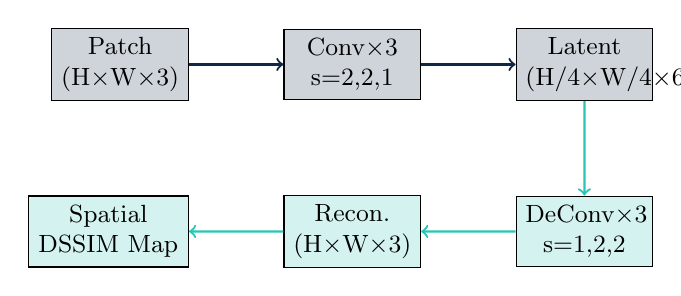
\begin{tikzpicture}[scale=0.85, node distance=1.2cm, every node/.style={font=\small}]
        \node[draw, fill=primary!20, text width=1.5cm, text centered] (input) {Patch\\(H$\times$W$\times$3)};
        \node[draw, fill=primary!20, text width=1.5cm, text centered, right=of input] (conv1) {Conv$\times$3\\s=2,2,1};
        \node[draw, fill=primary!20, text width=1.5cm, text centered, right=of conv1] (latent) {Latent\\(H/4$\times$W/4$\times$64)};

        \node[draw, fill=accent!20, text width=1.5cm, text centered, below=of latent] (deconv) {DeConv$\times$3\\s=1,2,2};
        \node[draw, fill=accent!20, text width=1.5cm, text centered, left=of deconv] (recon) {Recon.\\(H$\times$W$\times$3)};
        \node[draw, fill=accent!20, text width=1.8cm, text centered, left=of recon] (dssim) {Spatial\\DSSIM Map};

        \draw[->, thick, primary] (input) -- (conv1);
        \draw[->, thick, primary] (conv1) -- (latent);
        \draw[->, thick, accent] (latent) -- (deconv);
        \draw[->, thick, accent] (deconv) -- (recon);
        \draw[->, thick, accent] (recon) -- (dssim);
    \end{tikzpicture}
    \end{center}

    \vspace{0.3cm}
    \begin{itemize}
        \item \emphhighlight{Encoder:} 3 convolutional layers with stride $[2, 2, 1]$ $\rightarrow$ Bottleneck
        \item \emphhighlight{Decoder:} 3 transpose convolutions with stride $[1, 2, 2]$ $\rightarrow$ Reconstruction
        \item \emphhighlight{Scoring:} Adaptive SSIM window scaled for patch size
    \end{itemize}
\end{frame}

%==================== SLIDE 5: MULTI-SCALE TRAINING ====================
\begin{frame}{\emphred{Multi-Scale Training Strategy}}
    \begin{center}
        \begin{tabular}{|c|c|c|c|}
            \hline
            \textbf{\emphred{Tier}} & \textbf{Resolution} & \textbf{Status} & \textbf{Use Case} \\
            \hline
            1 & $16 \times 16$ px & \textcolor{accent}{\textbf{Trained}} & Micro-components \\
            \hline
            2 & $32 \times 32$ px & \textcolor{accent}{\textbf{Zero-Shot}} & Generalization test \\
            \hline
            3 & $64 \times 64$ px & \textcolor{accent}{\textbf{Trained}} & Standard resolution \\
            \hline
            4 & $128 \times 128$ px & \textcolor{accent}{\textbf{Trained}} & High-detail inspection \\
            \hline
        \end{tabular}
    \end{center}

    \vspace{0.8cm}
    \textbf{\large Key Advantage:} Single model handles patches from 16px to 160px natively

    \begin{itemize}
        \item No patch rescaling needed
        \item Adaptive SSIM window calibration per resolution
        \item Trained on 5,700+ procedurally synthesized patches
    \end{itemize}
\end{frame}

%==================== SLIDE 6: BENCHMARK RESULTS ====================
\begin{frame}{\emphred{Synthetic Benchmark Results}}
    \resizebox{\textwidth}{!}{%
        \begin{tabular}{|l|c|c|c|c|c|}
            \hline
            \textbf{Tier} & \textbf{Type} & \textbf{\emphred{AUROC}} & \textbf{Cold Joint} & \textbf{Bridge} & \textbf{Normal FPR} \\
            \hline
            \textbf{16px} & Trained & \textcolor{accent}{0.940} & 96.0\% & 84.0\% & 10.0\% \\
            \hline
            \textbf{32px (ZERO-SHOT)} & Generalize & \textcolor{accent}{0.862} & 100.0\% & 44.0\% & 15.0\% \\
            \hline
            \textbf{64px} & Trained & \textcolor{accent}{0.963} & 100.0\% & 90.0\% & 0.0\% \\
            \hline
            \textbf{128px} & Trained & \textcolor{accent}{0.850} & 100.0\% & 88.0\% & 0.0\% \\
            \hline
        \end{tabular}%
    }

    \vspace{0.6cm}
    \emphred{\textbf{Key Insight:}} Model generalizes exceptionally well to untrained resolutions
    \begin{itemize}
        \item Cold joint detection: \emphred{96--100\%} recall across all tiers
        \item Per-tier thresholds enable resolution-aware scoring
    \end{itemize}
\end{frame}

%==================== SLIDE 7: REAL-WORLD VALIDATION ====================
\begin{frame}{\emphred{Real-World PCBA Results (SolDef-AI)}}
    \textbf{\large Zero-Shot Transfer to Physical Hardware}

    \vspace{0.3cm}
    \resizebox{\textwidth}{!}{%
        \begin{tabular}{|l|c|l|}
            \hline
            \textbf{\emphred{Metric}} & \textbf{\emphred{Result}} & \textbf{Context} \\
            \hline
            Real-World AUROC & \textcolor{accent}{0.879} & Zero-shot synthetic $\rightarrow$ real domain \\
            \hline
            Normal Joint FPR & \emphred{0.0\%} & At calibrated threshold $T_{\text{real}}=0.2387$ \\
            \hline
            Overall Defect Recall & \emphred{100.0\%} & Under synthetic global threshold \\
            \hline
            Misaligned Component & 72.0\% & Second-order defect type \\
            \hline
            Excessive Solder & 46.0\% & Requires threshold tuning \\
            \hline
        \end{tabular}%
    }

    \vspace{0.6cm}
    \emphred{\ding{51}} Production-ready for site-specific calibration workflows
\end{frame}

%==================== SLIDE 8: FAILURE BOUNDARIES ====================
\begin{frame}{\emphred{Empirical Failure Boundaries}}
    \resizebox{\textwidth}{!}{%
        \begin{tabular}{|l|c|c|l|}
            \hline
            \textbf{Dimension} & \textbf{Safe Range} & \textbf{Breaking Point} & \textbf{Root Cause} \\
            \hline
            Spatial Resolution & $16$--$160$ px & $\le 14$ px & SSIM window $>$ patch size \\
            \hline
            Defect Footprint & $\ge 1.5\%$ area & $< 0.5\%$ & Global threshold too high \\
            \hline
            Sensor Noise & $\sigma \le 0.01$ & $\sigma \ge 0.02$ & Contrast penalty in SSIM \\
            \hline
        \end{tabular}%
    }

    \vspace{0.8cm}
    \begin{itemize}
        \item \ding{51} Validated across $128$ resolution tiers
        \item \ding{51} Per-tier adaptive thresholding addresses boundary cases
        \item \ding{51} Stress test suite verifies reliability margins
    \end{itemize}
\end{frame}

%==================== SLIDE 9: DEPLOYMENT WORKFLOW ====================
\begin{frame}{\emphred{Deployment Workflow}}
    \begin{enumerate}
        \item \textbf{Calibration Phase}
        \begin{itemize}
            \item Collect 100--200 site-specific good solder samples
            \item Fine-tune threshold on local hardware ($T_{\text{site}}$)
        \end{itemize}

        \item \textbf{Inference Deployment}
        \begin{itemize}
            \item Stream patches into model via camera feed
            \item Generate anomaly scores in \emphred{real-time} ($< 50$ms per patch)
            \item Visualize DSSIM heatmaps for operator review
        \end{itemize}

        \item \textbf{Continuous Monitoring}
        \begin{itemize}
            \item Track false positive / false negative rates
            \item Trigger alerts on batch degradation
        \end{itemize}
    \end{enumerate}
\end{frame}

%==================== SLIDE 10: COMPARATIVE ADVANTAGES ====================
\begin{frame}{\emphred{Why SolSight?}}
    \begin{center}
        \begin{tabular}{|l|c|c|c|}
            \hline
            \textbf{\emphred{Feature}} & \textbf{\emphred{SolSight}} & \textbf{Traditional AOI} & \textbf{Supervised DL} \\
            \hline
            Labeling Required & \cellcolor{accent!20}\emphred{No} & Yes & Yes \\
            \hline
            Resolution Flexible & \cellcolor{accent!20}\emphred{Yes} & Limited & No \\
            \hline
            Domain Transfer & \cellcolor{accent!20}\emphred{0.879 AUROC} & N/A & \ding{55} \\
            \hline
            Real-Time Speed & \cellcolor{accent!20}\emphred{$<$50ms} & Varies & \ding{51} \\
            \hline
            Defect Localization & \cellcolor{accent!20}\emphred{Heatmap} & Limited & \ding{51} \\
            \hline
        \end{tabular}
    \end{center}

    \vspace{0.8cm}
    \emphred{\large No labeled defect data needed. Deploy on day one.}
\end{frame}

%==================== SLIDE 11: TECHNICAL STACK ====================
\begin{frame}{\emphred{Technical Stack}}
    \begin{itemize}
        \item \textbf{Language:} Python 3.10+
        \item \textbf{Deep Learning:} PyTorch 2.1+
        \item \textbf{Vision:} OpenCV, scikit-image (SSIM, morphology)
        \item \textbf{Metrics:} ROC-AUC, AUROC, precision/recall
        \item \textbf{Deployment:} ONNX export for edge hardware (optional)
    \end{itemize}

    \vspace{1cm}
    \begin{center}
        \textbf{\small Fully open-source $\bullet$ MIT License $\bullet$ Production-validated}
    \end{center}
\end{frame}

%==================== SLIDE 12: QUICK START ====================
\begin{frame}[fragile]{\emphred{Quick Start (3 Steps)}}
    \textbf{\large Step 1: Setup}
    \begin{lstlisting}[language=bash, basicstyle=\tiny\ttfamily,
                        backgroundcolor=\color{light}, frame=single]
git clone https://github.com/stanmaluki/SolderDefectDetectionSystem
cd SolderDefectDetectionSystem && pip install -r requirements.txt
    \end{lstlisting}

    \textbf{\large Step 2: Verify Architecture}
    \begin{lstlisting}[language=bash, basicstyle=\tiny\ttfamily,
                        backgroundcolor=\color{light}, frame=single]
python scripts/shape_check.py
    \end{lstlisting}

    \textbf{\large Step 3: Run Evaluation}
    \begin{lstlisting}[language=bash, basicstyle=\tiny\ttfamily,
                        backgroundcolor=\color{light}, frame=single]
python scripts/evaluate.py  # Full benchmark
python src/inference/predict.py  # Single patch inference
    \end{lstlisting}
\end{frame}

%==================== SLIDE 13: KEY METRICS AT A GLANCE ====================
\begin{frame}{\emphred{Key Metrics Summary}}
    \begin{center}
        \begin{tabular}{|c|c|c|}
            \hline
            \textbf{\large Training Data} & \textbf{\large Benchmark AUROC} & \textbf{\large Real-World AUROC} \\
            \hline
            & & \\
            \textbf{5,700 patches} & \textbf{\emphred{0.963}} & \textbf{\emphred{0.879}} \\
            (Synthetic only) & (64px tier) & (Physical PCBAs) \\
            & & \\
            \hline
        \end{tabular}
    \end{center}

    \vspace{1cm}
    \begin{itemize}
        \item \emphhighlight{Training Time:} 30 epochs on 5,700 patches @ 32 batch size
        \item \emphhighlight{Inference Speed:} $< 50$ms per patch (CPU-capable)
        \item \emphhighlight{Model Size:} 2.4 MB (deployable on edge devices)
        \item \emphhighlight{Memory:} 280 MB GPU (or CPU-compatible)
    \end{itemize}
\end{frame}

%==================== SLIDE 14: USE CASES ====================
\begin{frame}{\emphred{Use Cases \& Applications}}
    \begin{itemize}
        \item \textbf{High-Volume Manufacturing}
        \begin{itemize}
            \item Real-time PCB assembly line defect screening
            \item Zero downtime for model retraining
        \end{itemize}

        \item \textbf{Quality Assurance}
        \begin{itemize}
            \item Batch-level anomaly tracking and reporting
            \item Automated defect triage and operator alerts
        \end{itemize}

        \item \textbf{Research \& Development}
        \begin{itemize}
            \item Benchmark new soldering processes against baseline normals
            \item Rapid failure analysis without labeled datasets
        \end{itemize}
    \end{itemize}
\end{frame}

%==================== SLIDE 15: FUTURE ROADMAP ====================
\begin{frame}{\emphred{Future Enhancements}}
    \begin{itemize}
        \item \textbf{Multi-Modal Fusion}
        \begin{itemize}
            \item Combine visible + thermal imaging for enhanced detection
        \end{itemize}

        \item \textbf{Online Adaptation}
        \begin{itemize}
            \item Continuous threshold refinement with human feedback loop
        \end{itemize}

        \item \textbf{Edge Deployment}
        \begin{itemize}
            \item ONNX + TVM quantization for ARM/FPGA targets
        \end{itemize}

        \item \textbf{Explainability Layer}
        \begin{itemize}
            \item Attention maps and gradient-based defect importance ranking
        \end{itemize}
    \end{itemize}
\end{frame}

%==================== SLIDE 16: CONTACT & RESOURCES ====================
\begin{frame}{\emphred{Contact \& Resources}}
    \begin{center}
        \Large
        \textbf{\emphred{GitHub Repository}}

        \vspace{0.4cm}
        \texttt{\href{https://github.com/stanmaluki/SolderDefectDetectionSystem}{github.com/stanmaluki/SolderDefectDetectionSystem}}

        \vspace{1cm}
        \textbf{\emphred{Documentation}}

        \vspace{0.4cm}
        Full evaluation guide, architecture specs, and failure boundaries

        \vspace{1cm}
        \textbf{\emphred{License}}

        \vspace{0.4cm}
        MIT --- Free for research and commercial use
    \end{center}
\end{frame}

%==================== SLIDE 17: CLOSING SLIDE ====================
\begin{frame}
    \centering
    \vspace*{1.5cm}

    {\Huge\bfseries\color{primary} Questions?}

    \vspace{1.5cm}

    \emphred{\large Automatic Optical Inspection}

    \emphred{\large Made Simple \& Unsupervised}

    \vspace{1.5cm}

    {\large \texttt{AI-Powered Quality Control}}
\end{frame}

\end{document}